\documentclass[12pt]{article}

% Language setting
% Replace `english' with e.g. `spanish' to change the document language
\usepackage[english]{babel}

% Set page size and margins
% Replace `letterpaper' with `a4paper' for UK/EU standard size
\usepackage[letterpaper,top=2cm,bottom=2cm,left=3cm,right=3cm,marginparwidth=1.75cm]{geometry}

% Useful packages
\usepackage{amsmath}
\usepackage{graphicx}
\usepackage[colorlinks=true, allcolors=blue]{hyperref}

\title{Title: Preventive Maintenance of Industrial Rotational Machinery through Machine Learning and Audio Analysis}
\author{You}

\begin{document}
\maketitle

\begin{abstract}
Your abstract.
\end{abstract}

%%%--- HARDWARE PLATFORM
\section{Hardware Platform}

Texas Instruments’ SK-AM62A-LP

%%%--- EXPLANATION OF IDEA
\section{Explanation of the Idea}
% Include a block diagram, overview of implementation  (Minimum font size: 10pt, Times New Roman font. Maximum two pages including tables, diagram, references (if any) )

High-performance rotational machinery is crucial to numerous industrial fields such as rolling mills, turbines, and raw material processing.
A recent study of more than 400 malfunctioning of just one type of pumps, multistage centrifugal pumps (MCPs), found that the industry suffered more than 6000 hours of maintenance-related downtime due to the absence of precise and intelligent fault diagnosis (FD), incurring a cost in the range of 50 million USD \cite{rane2021re}.
The vast array of uses for rotational machinery implies that malfunctions can lead to major repercussions, such as energy waste, industrial process interruptions, financial losses, costly repairs, and jeopardized employee safety. 

To maintain dependable operation, early fault detection is important and should minimize maintenance and repair expenses. Consistent supervision can be achieved using affordable and reliable signal processing and artificial intelligence (AI) techniques \cite{sunal2022review}. AI techniques for fault detection involve preprocessing signals and features to identify and classify faults \cite{saeed2021fault, jiang2019bearing}.

\begin{figure}
\centering
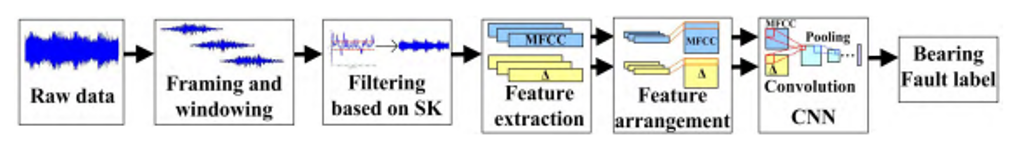
\includegraphics[width=0.9\linewidth]{figs/fig-arch1.png}
\caption{\label{fig:arch1}Proposed architecture of the fault detection using audio analytics and machine learning.}
\end{figure}




\section{Example of its Application}
% application (Describe an example consisting of potential application/Future application. This will enable usage model towards its market acceptance) (maximum 200 words)

\section{Benefits and Value Addition}
% (Explain the key benefits of your idea/implementation. You should describe the key value addition of your idea as this will explain why your idea has value in the presence of other participants. It will show uniqueness/Unique selling point/key differentiator) (maximum 200 words)

\section{Team Members}
% •	List your team members’ names, program, department, year of study and contact emails here

\section{University Address}
% •	Include the name of your university/college and your institute’s postal address to ship the boards

\section{Contact Person}
% •	Mention one contact person from the institute, his/her official/institute email id, and contact phone number.

\bibliographystyle{ieeetr}
\bibliography{sample}

\end{document}